\chapter{Anforderungen}
\label{cha:Anforderungen}

An Cloud-Systeme wird, mit oder ohne Kubernetes, eine Vielzahl an Anforderungen
gestellt.
Im Folgenden werden diese genannt und genau definiert, um in der Analyse
beurteilen zu können, ob diese erreicht werden.

\section{Kosten}

\subsection{Infrakstruktur-Kosten}
Hierunter fallen die Kosten für den Betrieb der Dienste bei den IaaS-Anbietern.
Um schließlich geringere Server-Kosten zu erzielen, muss mit der Migration erst
eine
Investition getätigt werden, denn beide Systeme werden während der Migration parallel laufen
müssen.
Sobald die Migration beendet ist, sollten die neuen Kosten geringer sein und
sich damit dann auch die getätigte Investition durch Einsparungen wieder ausgleichen.

\begin{figure}[H]
\centering
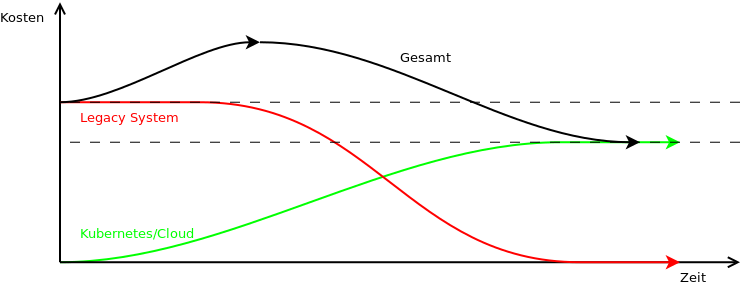
\includegraphics[width=1\textwidth]{kosten}
\caption{Schematische Darstellung der gewünschten Kostenentwicklung}
\end{figure}

% \subsection{Personalkosten}
% Es sind aber auch Kosten gemeint, wie die Gehälter der Mitarbeiter,
% die für die Implementation und den Betrieb dieser Dienste verantwortlich sind.
% Desto geringer die Komplexität des Systems, desto weniger Mitarbeiter müssen sich
% mit dieser Aufgabe auseinandersetzen.
% Da diese Faktoren aber im Rahmen eines fiktiven Case-Studies schwer zu bemessen sind,
% sollen sie an dieser Stelle nur Erwähnung finden. Eine spätere Auswertung kann
% hier nur geschätzt werden.

\subsection{Kosten für externe Tools}
Desto weniger externe Dienste von SaaS-Anbietern benutzt
werden, desto mehr Kosten können eingespart werden.
Statt bei einem externen Dienstleister, laufen diese Dienste dann auf der eigenen
Infrastruktur.

\section{Sicherheit}

\subsection{Betriebssystem-Patches}
Um vor Sicherheitslücken durch das Betriebssystem gefeit zu sein,
empfiehlt es sich, die Betriebssystem-Version immer möglichst aktuell zu halten.

\subsection{Ports}
Nach außen hin offene Ports müssen ausreichend abgesichert sein. Das bedingt,
dass nicht benötigte Ports geschlossen werden, aber auch, dass die offenen Ports
entsprechend abgesichert sind.

\subsection{Verschlüsselung}
Die Kommunikation des Clusters mit seinen Clients sollte mittels Transport
Layer Security (TLS) abgesichert werden, um Man-in-the-middle Attacken
zu verhindern.

\subsection{Authentifizierung und Autorisierung}
Es soll sichergestellt sein, dass der Benutzer, der sich mit dem System verbindet,
auch wirklich der Benutzer ist, der er vorgibt zu sein.
Die authentifizierten Benutzer sollen nur Zugang zu den Schnittstellen haben,
die sie auch wirklich benutzen dürfen.

\subsection{Interne Angriffsvektoren}
Auch innerhalb des Systems sollten Angriffsvektoren möglichst vermieden werden.
Dienste sollten deshalb möglichst abgekapselt voneinander laufen und nur die
Rechte auf
andere Dienste bekommen, die sie auch wirklich brauchen.
Sollte ein Angreifer über eine Sicherheitslücke Zugriff bekommen, ist damit
nicht das gesamte System kompromittiert.

\section{Automatische Skalierung}
Das Bereithalten von Infrastruktur, die dann aber nicht komplett ausgelastet wird,
ist teuer und sollte vermieden werden.
Die zur Verfügung stehenden Ressourcen sollten sich an der Nachfrage nach eben
diesen orientieren
und entsprechend hinzuschalten oder terminieren.

In folgender Grafik sieht man schematisch, wie ein System mittels automatischer
Skalierung,
Ressourcen bereit stellt, sollten diese benötigt werden.

\begin{figure}[H]
\centering
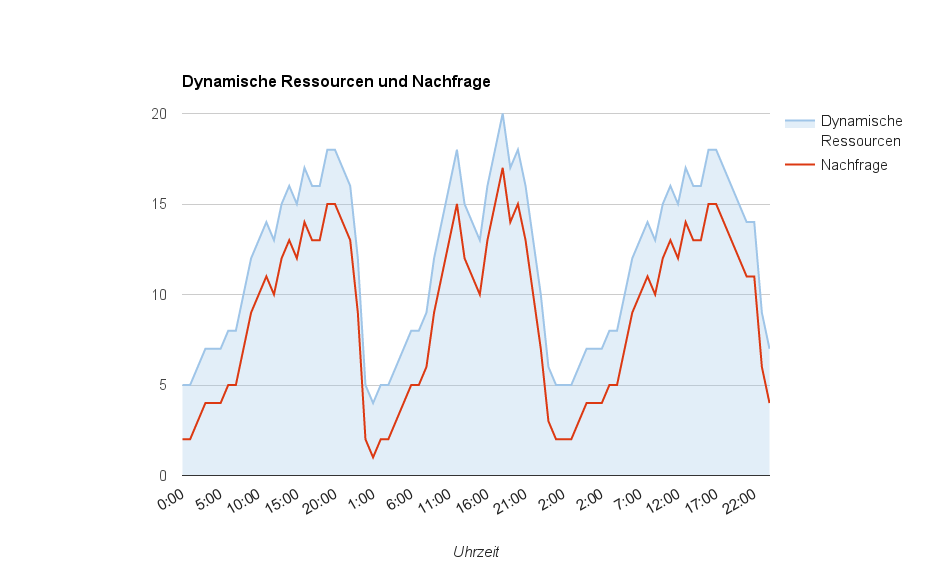
\includegraphics[width=1\textwidth]{dynamisch}
\caption{Beispielhafte Darstellung von dynamischen Ressourcen und Nachfrage}
\end{figure}

Im Vergleich dazu, ein System, das nicht skaliert, sondern statisch auf ein
geschätztes Maximum, Ressourcen bereit hält.
Die Fläche zwischen den Ressourcen und der Nachfrage stellt den verschwendeten
Aufwand dar \cite{masteroslo}. Sollte entgegen der Schätzung
des Maximums nun doch mehr Last auf diesem System liegen, k\"onnte
diese Last nicht mehr verarbeitet werden. Eine dynamische Skalierung könnte
Last jedoch auch dann noch abfangen.

\begin{figure}[H]
\centering
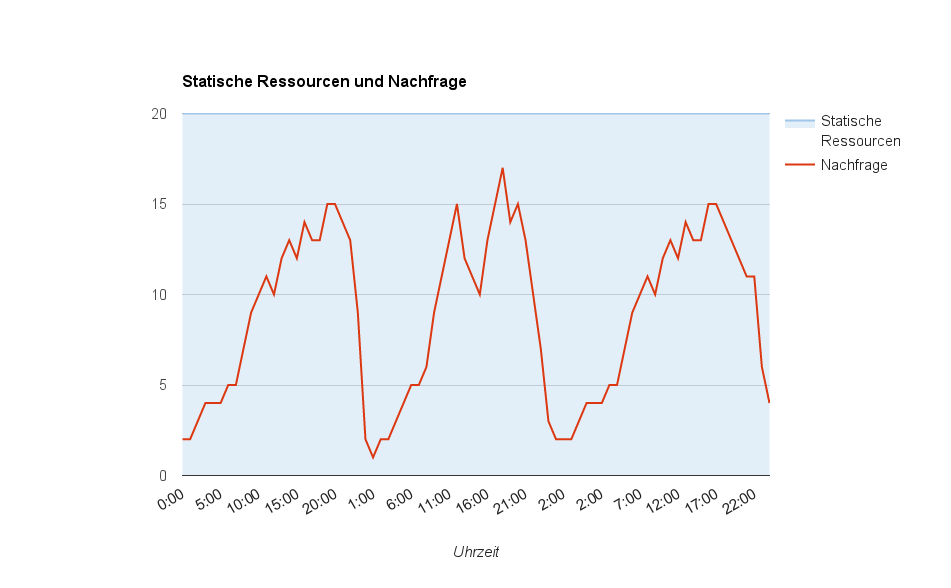
\includegraphics[width=1\textwidth]{statisch}
\caption{Beispielhafte Darstellung von statischen Ressourcen und Nachfrage}
\end{figure}

\section{Vendor Lock-in vermeiden}
Auf dem IaaS-Markt gibt es eine Reihe von Anbietern, die miteinander
konkurrieren, sodass sich
Preise und Leistungen ständig verändern.
Um von den, sich stätig verbessernden Konditionen auf dem Markt, profitieren
zu können,
empfiehlt es sich, darauf zu achten, dass keine Bindung an einen speziellen
IaaS-Anbieter eingegangen wird.
Eine Bindung entsteht in der Regel dann, wenn die Benutzung von Funktionalität
eines Anbieters über eine nicht standardisierte Schnittstelle erfolgt oder, wenn
Produkte genutzt werden, die in dieser Form
nicht auch bei anderen Anbietern vorhanden sind.
Bei einem Wechsel würden dann weitere Aufwendungen für die Anpassung
an die jeweils neuen Schnittstellen anfallen.

\section{Open Source statt proprietärer Software}
Open Source ist der Verwendung von proprietärer Software vorzuziehen.

Open Source Alternativen haben in der Regel folgende Vorteile:
\begin{itemize}
  \item Es muss keiner kompilierten Black-Box vertraut werden,
  denn die Funktionsweise von Open Source ist per Definition einsehbar.
  \item Es gibt die Möglichkeit, Implementierungsdetails an den eigenen Use Case
  anzupassen.
  \item Die Software steht kostenlos zur Verfügung.
\end{itemize}

\section{Self Hosted statt externe Provider}
Viele der Peripherie-Services, die für das Management einer Server-Infrastruktur
benötigt werden,
stehen auch als Open Source-Projekte zur Verfügung und in manchen Fällen
auch in fertigen Docker Base-Images.
Wenn man in der Lage ist, diese Services selbst zu hosten, entfallen die
Kosten für etwaige externe Dienste.
Ziel soll es deshalb sein, so viel wie möglich selbst zu hosten und auf externe
Dienste zu verzichten.
Ein weiterer großer Vorteil, wenn diese Services selbst gehostet werden, ist,
dass auch die
anfallenden Daten nicht bei einem externen Dienstleister liegen. So liegt auch
der Datenschutz für diese Daten in eigener Hand
und Maßnahmen können gemäß des jeweiligen Use Cases individuell durchgeführt
werden.


\section{Infrastructure as Code}
Im Gegensatz zum Definieren der Infrastruktur über eine GUI der IaaS-Anbieters,
steht die Konfiguration über APIs des Anbieters.
Diese bietet folglich die Möglichkeit diese Schnittstellen mittels Code anzusteuern.
Ist die Infrastruktur als Code beschrieben, bieten sich folgende Vorteile:

\begin{itemize}
  \item Wiederholbare Deployments
  \item Deterministische Deployments
  \item Versionierbare Infrastruktur
  \item Schneller als manuelle Konfiguration über eine GUI
  \item Verringerung des Vendor Lock-ins
\end{itemize}

\section{Ausfallsicherheit}
Um es mit den Worten von Werner Vogels, dem CTO von Amazon.com, zu sagen:
\quotes{Everything fails, all of the time.} \cite{everythingfails}.
Der beste Weg, um ausfallsichere Infrastruktur zu bauen,
ist deshalb, davon auszugehen, dass Komponenten potentiell jederzeit
ausfallen können.

Im Wesentlichen bedeutet diese Erkenntnis,
dass Redundanzen an kritischen Stellen geschaffen werden müssen.
Zusätzlich ist es wünschenwert, dass ein System, in dem es einen Ausfall gab,
automatisch wieder in einen funktionalen Zustand kommt.

\section{Disaster Recovery}
Falls die Infrastruktur komplett oder teilweise ausfällt,
braucht es schnelle und einfache Wege, um dafür zu sorgen, dass die Infrastruktur
wieder in Betrieb kommt. Hier geht es auch darum, dass Stateful Services (wie Datenbanken)
mit den letzten validen Daten wiederhergestellt werden können.

\section{Deployment Pipeline}
Die Deployment-Pipeline soll in den Workflow der Entwickler integriert sein.
Die Entwickler sollen, mit minimalen Aufwand, in der
Lage sein, eine neue Version zu deployen oder ein Roll-Back zu machen.
Die Veränderung auf dem Server soll dann zeitnah sichtbar sein.

\section{Geschwindigkeit}
Schnelle Ladezeiten der Website und der API tragen zur Zufriedenheit des
Benutzers bei.
Aus diesem Grund sollte das System, selbst unter Last, möglichst schnell Ergebnisse
liefern.

\section{Alerting}
Sollte es zu Ausfällen kommen, müssen die relevanten Personen darüber
informiert werden.
Das System muss also die Möglichkeit bieten, auf Grundlage von diversen Metriken,
Nachrichten zu versenden.

\section{Logging}
Die Applikationen, die auf dem Cluster laufen, werden Output auf \code{stdout}
und \code{stderr} loggen.
Dieser Output soll einfach einsehbar sein, sodass auch Entwickler darauf
zugreifen können, ohne mittels \code{ssh} auf die jeweilige Maschine gehen zu
müssen.
Zudem sollte es die Möglichkeit geben, mittels Queries auf bestimmte Logs
zuzugreifen.
So können Logdaten gezielt aufgerufen und analysiert werden, anstatt diese
in den oft großen Logdateien zu suchen.

\section{Monitoring}
Es muss eine Oberfläche zur Verfügung stehen, mit der Daten wie CPU-, Memory-, Netzwerk-, oder Festplatten-Metriken
übersichtlich und zusammengefasst einsehbar sind. So können Probleme, die sich
erst auf längere Zeit entfalten,
wie Memory Leaks, frühzeitig erkannt und beseitigt werden. Auch, wenn diese
Probleme ohne Vorwarnung trotzdem auftreten, helfen diese Daten oft,
die Ursachen im
Nachhinein zu finden.
Zudem ergibt sich daraus auch eine bessere Entscheidungsgrundlage,
für die Nachrüstung von Hardware.

\section{The 12-Factor App}
Unter dem Namen \quotes{The 12-Factor App} hat der PaaS-Provider \quotes{Heroku} eine Reihe
an Regeln und Best-Practices herausgegeben. Diese beschreiben, wie moderne
Web-Applikationen auszusehen haben, damit sie sich in das Paradigma der
containerbasierten Server-Cluster einfügen lassen. \cite{12factor}

\begin{description}
  \item[1. Codebase:]
  Die Codebase einer App sollte in einem Versionsmanagement-System eingecheckt sein.
  Aus diesem sollten möglichst regelmäßige Deployments in die unterschiedlichen
  Entwicklungsumgebungen (Staging, Production usw.) stattfinden.
  \item[2. Dependencies:]
  Die Dependencies, die die App benötigt, sollten explizit definiert sein.
  Als gutes Beispiel dienen hier das \code{Gemfile} in \emph{Ruby} oder die
  \code{package.json} in \emph{NodeJS}, welche diese Dependencies beschreiben.
  Betriebssystem-spezifische Abhängigkeiten können dann im Dockerfile definiert
  werden.
  \item[3. Konfiguration]
  Die Konfiguration der Applikation soll möglichst mit Umgebungsvariablen
  stattfinden. Auf keinen Fall jedoch in der Codebase selbst.
  \item[4. Backing Services:]
  Backing services sollten als angehängte Ressourcen behandeln werden, damit
  diese leicht austauschbar sind.
  \item[5. Build, release, run:]
  Die Vorgänge Build, Release und Run sollten voneinander getrennt sein.
  \item[6. Prozesse:]
  Die Applikation soll als Prozess ausgeführt werden.
  Sie soll keinen State speichern, der nicht auch verloren gehen darf. State sollte
  ausschließlich in den Persistenz-Services, wie Datenbanken, abgelegt werden.
  \item[7. Port binding:]
  Services werden über unterschiedliche Ports exponiert.
  \item[8. Concurrency:]
  Skalierung soll mittels des \emph{Prozess-Modells} passieren. Es sollte ein
  Prozess-Manager verwendet werden, anstatt Daemons oder PID-Files.
  \item[9. Disposability:]
  Die Applikation sollte schnell starten und stoppen.
  \code{SIGTERM} sollte
  möglichst schnell umgesetzt werden, ohne zum Beispiel aktive Requests einfach
  abzubrechen
  oder einen aktiven Job nicht zurück in eine Queue zu schreiben.
  \item[10. Parität der Environments:]
  Die Development-, Staging- und Production-Environments sollten immer so ähnlich wie möglich sein,
  um Vergleichbarkeit zu wahren und damit Fehlern in der Production-Environment
  vorzubeugen.
  \item[11. Logs:]
  Logs sollten als Stream von Events behandelt werden und ungebuffered
  auf \code{stdout} oder \code{stderr} schreiben.
  \item[12. Admin-Prozesse:]
  Admin/Management-Aufgaben, wie Datenbank-Migrationen, sollen
  als einmalige Vorgänge behandelt werden, die in der Applikations-Umgebung
  stattfinden.
\end{description}

Es soll untersucht werden, inwiefern diese Regeln im Zusammenhang mit Kubernetes
funktionieren und wie sie sich anwenden lassen.
